% !TEX program = xelatex
\documentclass[12pt,a4paper]{article}

% === 中文与字体 ===
\usepackage[fontset=windows]{ctex}
\usepackage{geometry}
\geometry{left=2.2cm,right=2.2cm,top=2.2cm,bottom=2.4cm}

% === 数学与符号 ===
\usepackage{amsmath,amssymb}
\usepackage{booktabs}
\usepackage[justification=centering]{caption}
\usepackage[unicode]{hyperref}
\hypersetup{hidelinks}

% === 图片 ===
\usepackage{graphicx}
\graphicspath{{../output/figures/}}
\usepackage{subcaption}

% === 标题与段落 ===
\usepackage{titlesec}
\titleformat{\section}{\large\bfseries}{\thesection.}{1em}{}
\titleformat{\subsection}{\normalsize\bfseries}{\thesubsection.}{1em}{}
\titlespacing*{\section}{0pt}{1.2ex}{0.8ex}
\titlespacing*{\subsection}{0pt}{1ex}{0.5ex}
\setlength{\parindent}{2em}
\setlength{\parskip}{0.3ex}

% === 页眉页脚 ===
\usepackage{fancyhdr}
\pagestyle{fancy}
\fancyhf{}
\fancyhead[C]{}
\fancyfoot[C]{\thepage}

\begin{document}

\title{\textbf{基于 LSTM 的中文文本分类与情感分析对比研究}}
\author{}
\date{}
\maketitle
\thispagestyle{fancy}

% ============================================================
\section{引言}
% ============================================================

随着互联网新闻数据的爆炸式增长，如何有效地对海量文本进行自动分类与情感分析已成为自然语言处理领域的重要课题。文本分类旨在将文档自动划分到预定义的类别中，而情感分析则关注文本所表达的情感倾向。二者在舆情监测、信息推荐、智能问答等场景中均有广泛应用，且具有天然的互补性：分类提供文本的主题信息，情感分析提供文本的态度信息，二者结合能够更全面地理解文本内容。

近年来，基于深度学习的文本分类方法取得了显著进展。其中，长短期记忆网络（LSTM）因其对序列数据的建模能力，在文本分类任务中表现出色。与此同时，基于情感词典的方法因其无需标注数据和计算资源较少的特点，仍被广泛用于情感分析任务。将这两种方法进行对比分析，有助于深入理解不同技术路线在同一数据集上的表现差异。

本研究以 THUCNews 中文新闻数据集为对象，以 LSTM 文本分类为主任务，Naive Bayes + TF-IDF 为基线对比，同时使用大连理工情感词汇本体库（DUTIR）进行情感分析，最终将分类结果与情感分析结果进行综合对比讨论。本文旨在探究三方面问题：(1) LSTM 在中文短文本分类中的有效性；(2) 传统方法（Naive Bayes）与深度方法（LSTM）的性能差距；(3) 不同新闻类别的情感分布特征及其与分类性能的关联。

% ============================================================
\section{数据与方法}
% ============================================================

\subsection{THUCNews 数据集}

本文采用清华大学发布的 THUCNews 数据集的十类别子集，包含 finance（财经）、realty（房产）、stocks（股票）、education（教育）、science（科技）、society（社会）、politics（政治）、sports（体育）、game（游戏）、entertainment（娱乐）共 10 个新闻类别。数据集共 200{,}000 条样本，划分为训练集 180{,}000 条、验证集 10{,}000 条和测试集 10{,}000 条，各类别样本数量均衡，每条样本为一条新闻标题。

\subsection{数据预处理与探索性分析}

原始数据以 \texttt{文本\t标签} 的格式存储。预处理流程如下：首先对文本进行清洗，保留中文字符、英文字母和数字；接着使用 jieba 分词工具进行中文分词，并去除停用词；然后基于训练集构建词汇表，设定最大词汇量为 50{,}000，最低词频为 5，最终词汇表大小为 30{,}601；最后将文本序列编码为索引序列。

\begin{figure}[htbp]
\centering
\begin{subfigure}[b]{0.46\textwidth}
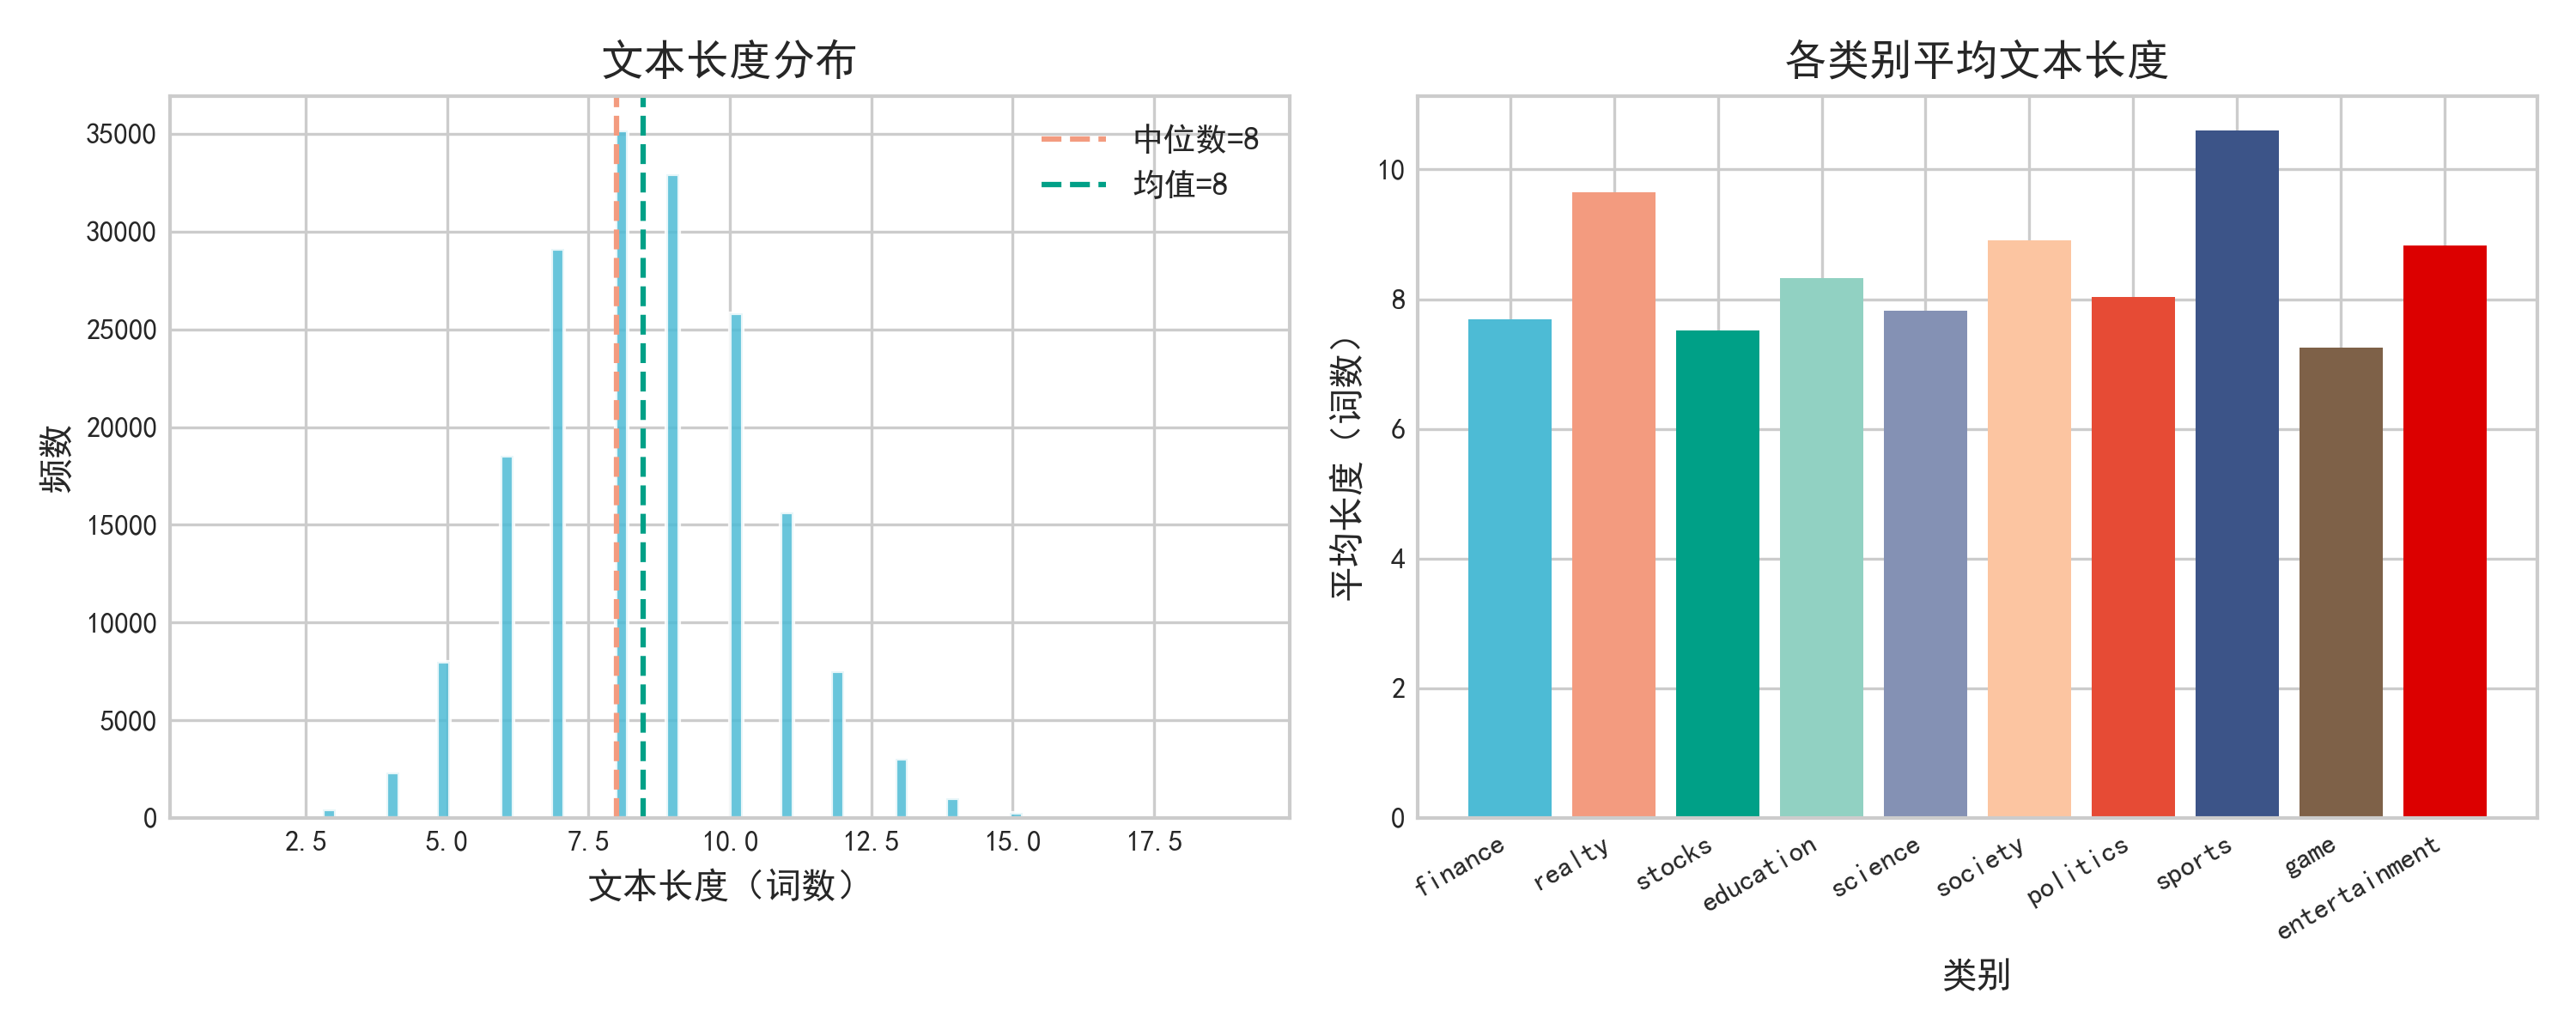
\includegraphics[width=\textwidth]{fig1_text_length_dist.png}
\caption{文本长度分布}
\label{fig:length}
\end{subfigure}
\begin{subfigure}[b]{0.46\textwidth}
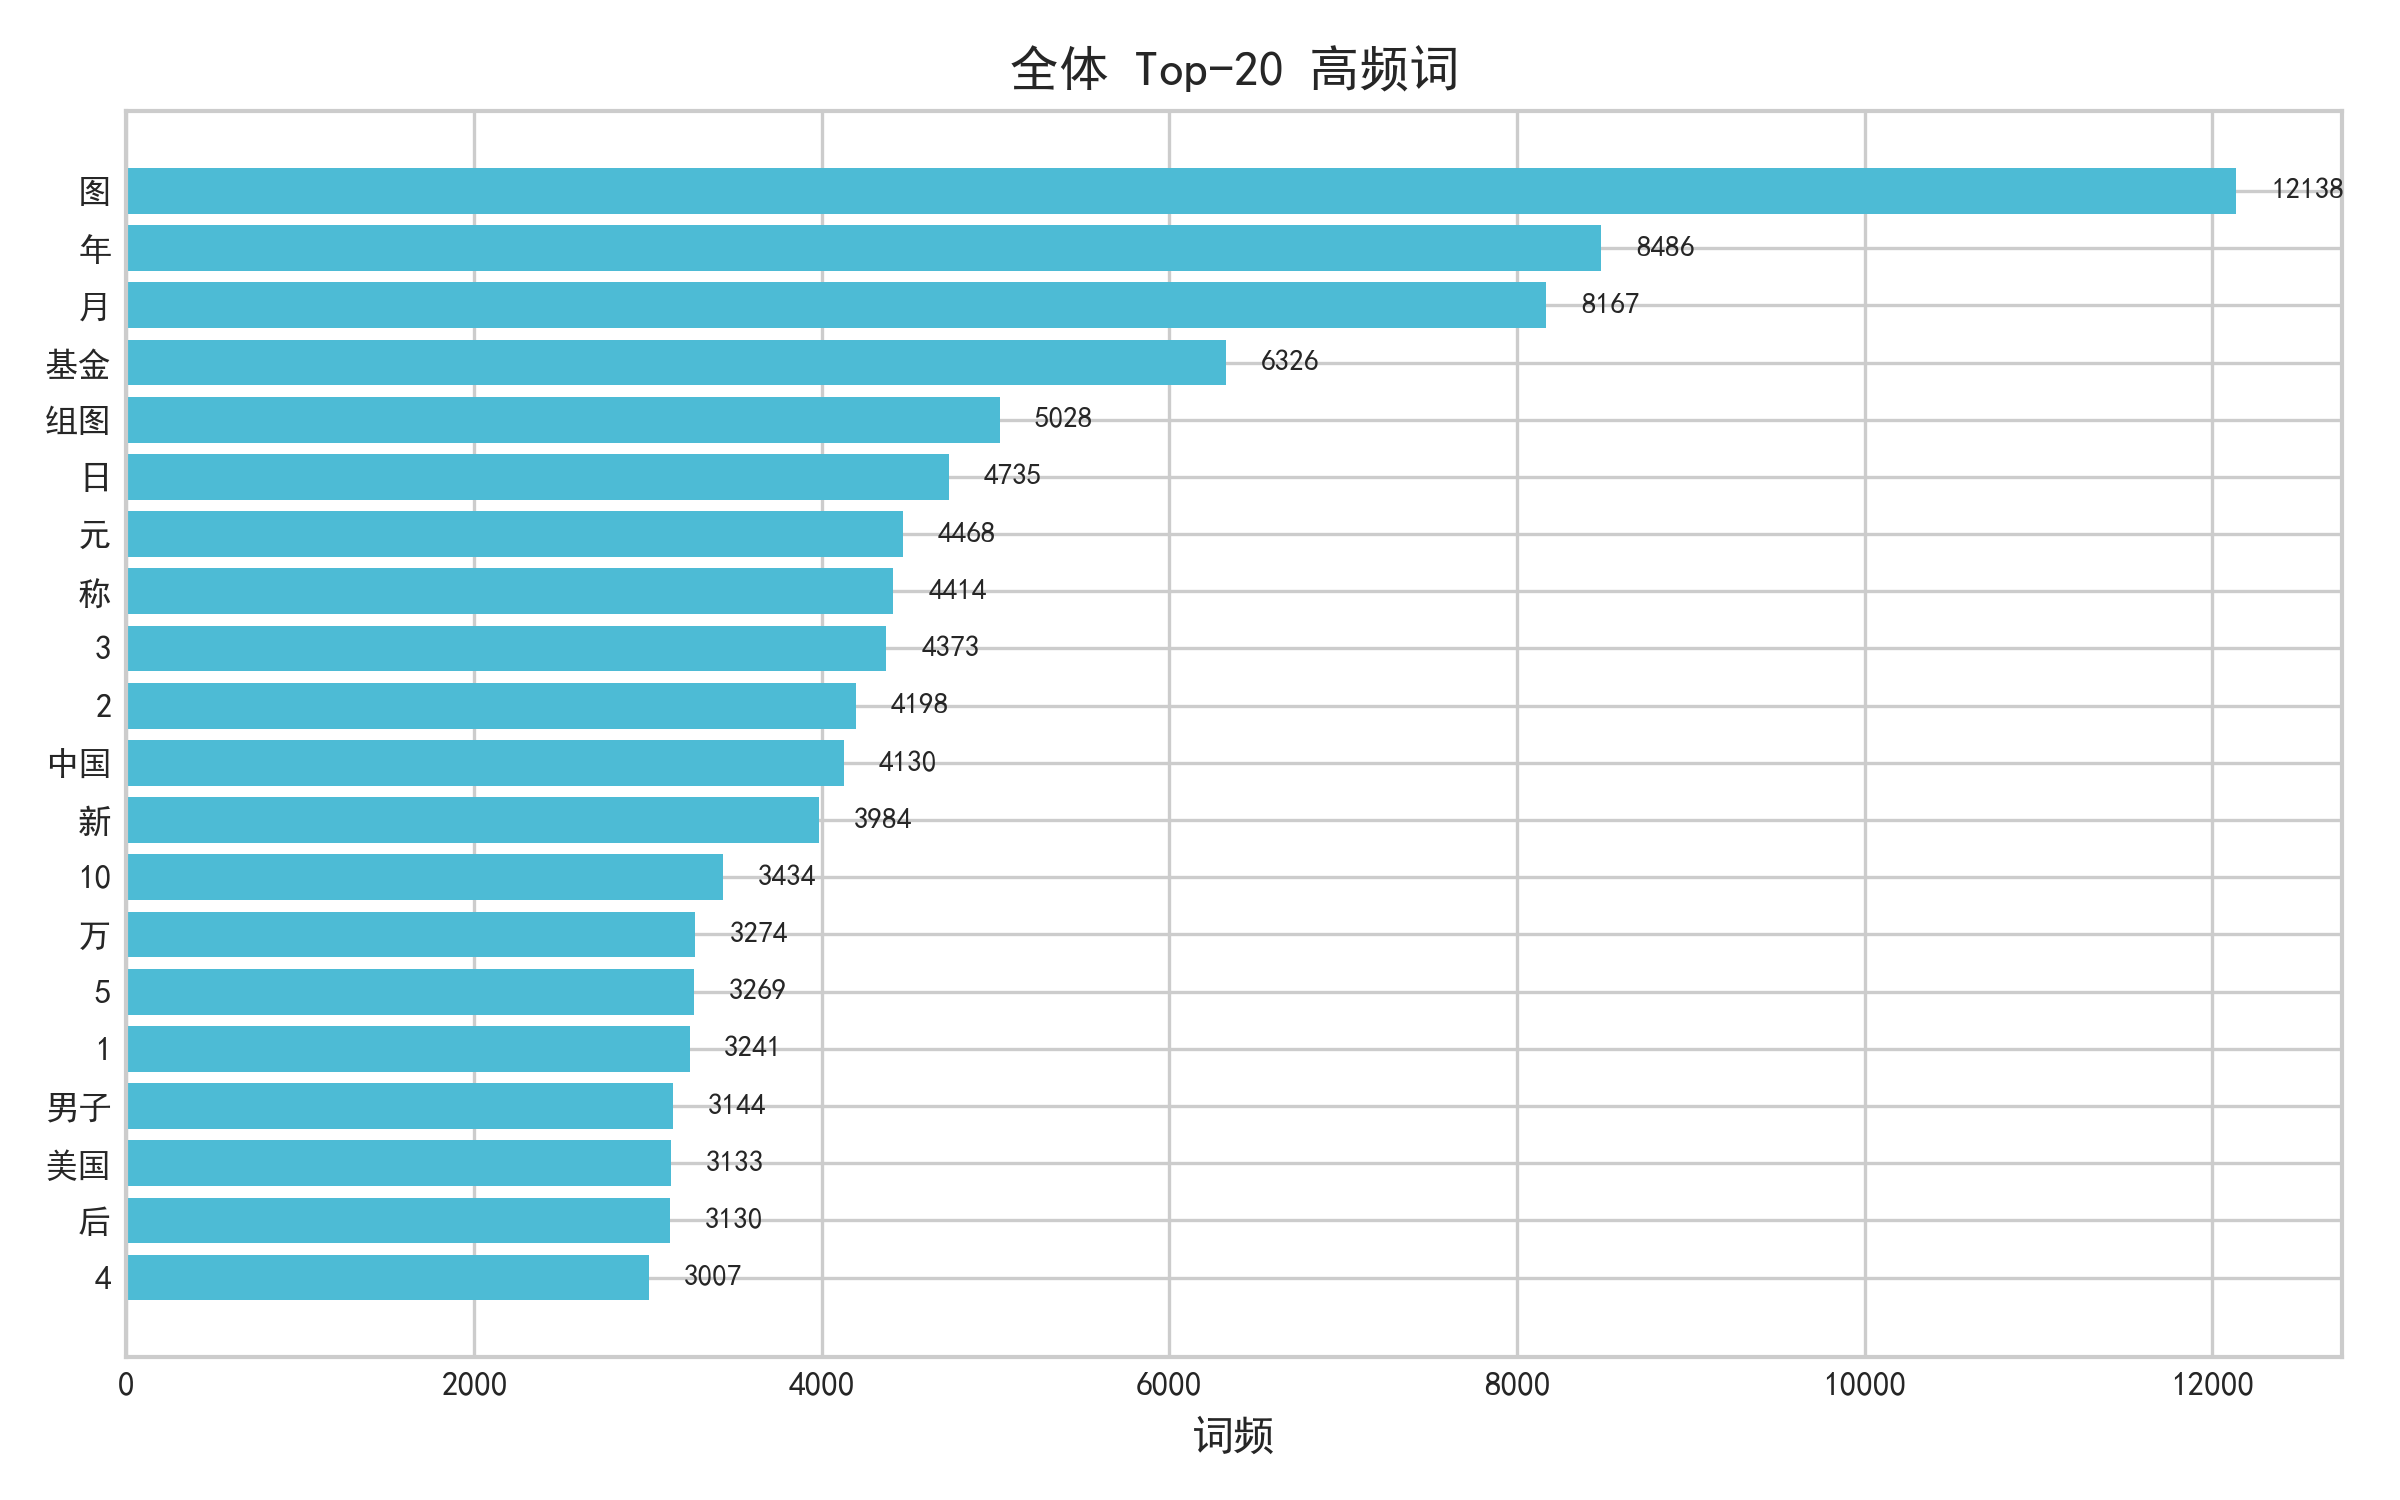
\includegraphics[width=\textwidth]{fig3_top_words.png}
\caption{全体 Top-20 高频词}
\label{fig:topwords}
\end{subfigure}
\caption{数据集探索性分析}
\label{fig:eda}
\end{figure}

图~\ref{fig:length} 展示了训练集的文本长度分布情况。文本长度的均值为 8.46 个词，中位数为 8 个词，最大不超过 20 个词，表明 THUCNews 数据集的文本以短文本（新闻标题）为主。各类别的平均文本长度略有差异，但总体分布较为一致。图~\ref{fig:topwords} 显示了全体数据中的 Top-20 高频词，其中"图"（图片新闻常用前缀）、"年"（时间词）、"日"（时间词）、"公司"（财经类关键词）、"中国"（国名）等词出现频率最高，这些高频词反映了新闻文本的典型用语特征。

\subsection{Word2Vec 词向量}

本文采用 Word2Vec Skip-gram 模型在训练集上进行无监督词向量训练。词向量维度设为 200，上下文窗口为 5，最低词频为 5，采用负采样策略（负采样数 10），迭代 10 轮。训练共耗时 55 秒，获得 30{,}599 个词的向量表示，覆盖词汇表全部词语。预训练的词向量作为 LSTM 嵌入层的初始权重，在训练过程中进行微调。

从词向量相似性来看，语义相近的词在向量空间中呈现出聚类特征。例如，"中国"的最近邻词包括"新华社"、"外交部"、"海峡"等与国家政治新闻相关的词汇；"教育"的最近邻词包括"高等教育"、"素质教育"等教育相关词汇；"游戏"的最近邻词包括"网游"、"玩家"、"FPS"等游戏领域术语。这表明训练得到的词向量较好地捕捉了词语的语义信息。

\subsection{LSTM 文本分类模型}

LSTM（Long Short-Term Memory）是一种特殊的循环神经网络，通过引入遗忘门、输入门和输出门，有效缓解了传统 RNN 中的梯度消失和梯度爆炸问题。对于文本分类任务，LSTM 能够捕捉文本中的长距离依赖关系，提取序列的上下文特征。

本文搭建的 LSTM 分类模型结构如下：首先使用预训练的 Word2Vec 词向量初始化嵌入层（维度 200），嵌入层在训练过程中进行微调；接着接入单层 LSTM 层，隐藏单元数分别为 64 和 128（两种配置）；然后对 LSTM 所有时间步的输出进行基于掩码的平均池化，以聚合序列信息、避免填充位对结果的干扰；最后通过 Dropout 层（丢弃率 0.5）和全连接层输出 10 个类别的概率分布。

模型训练采用 Adam 优化器，学习率为 0.01，批大小为 128，最大训练轮次为 20，并采用早停策略（验证损失连续 4 轮不下降则停止）。为加速 CPU 训练，对训练集按类别等比例采样至每类 3{,}000 条（共 30{,}000 条），序列长度截断至 50。

\subsection{情感分析方法}

本文采用基于情感词典的方法进行情感分析，具体使用大连理工大学信息检索研究室构建的情感词汇本体库（DUTIR），通过 Python 的 cnsenti 库调用。该词典包含 27{,}000 余个情感词汇，涵盖乐、好、怒、哀、惧、恶、惊 7 大类情感，并标注了情感强度与极性。情感分析流程为：对每条文本统计正面情感词和负面情感词数量，根据两者比较判定文本的情感极性（正面、负面或中性）。

% ============================================================
\section{实验与结果}
% ============================================================

\subsection{文本分类结果}

\begin{table}[htbp]
\centering
\caption{分类模型性能对比}
\label{tab:results}
\begin{tabular}{lccc}
\toprule
模型 & 准确率 & F1 (macro) & 训练时间 \\
\midrule
LSTM (h=64, d=0.5) & 0.8845 & 0.8845 & 87.6s \\
LSTM (h=128, d=0.5) & 0.8790 & 0.8791 & 143.0s \\
Naive Bayes + TF-IDF & 0.2959 & 0.2937 & 1.9s \\
\bottomrule
\end{tabular}
\end{table}

表~\ref{tab:results} 展示了各模型在测试集上的分类性能。LSTM 模型在两个配置下均取得了接近 88\% 的分类准确率，其中隐藏单元数为 64 的配置表现最佳，测试准确率和 F1 值均为 0.8845。相比之下，Naive Bayes + TF-IDF 基线的准确率仅为 29.59\%，这主要是因为 THUCNews 数据集中的文本经过 jieba 分词后特征维度较高，且各类别之间存在较多共享词汇（如"中国"、"年"、"公司"等高频词在各类别中普遍出现），朴素贝叶斯的特征独立性假设在此场景下难以满足。

\begin{figure}[htbp]
\centering
\begin{subfigure}[b]{0.46\textwidth}
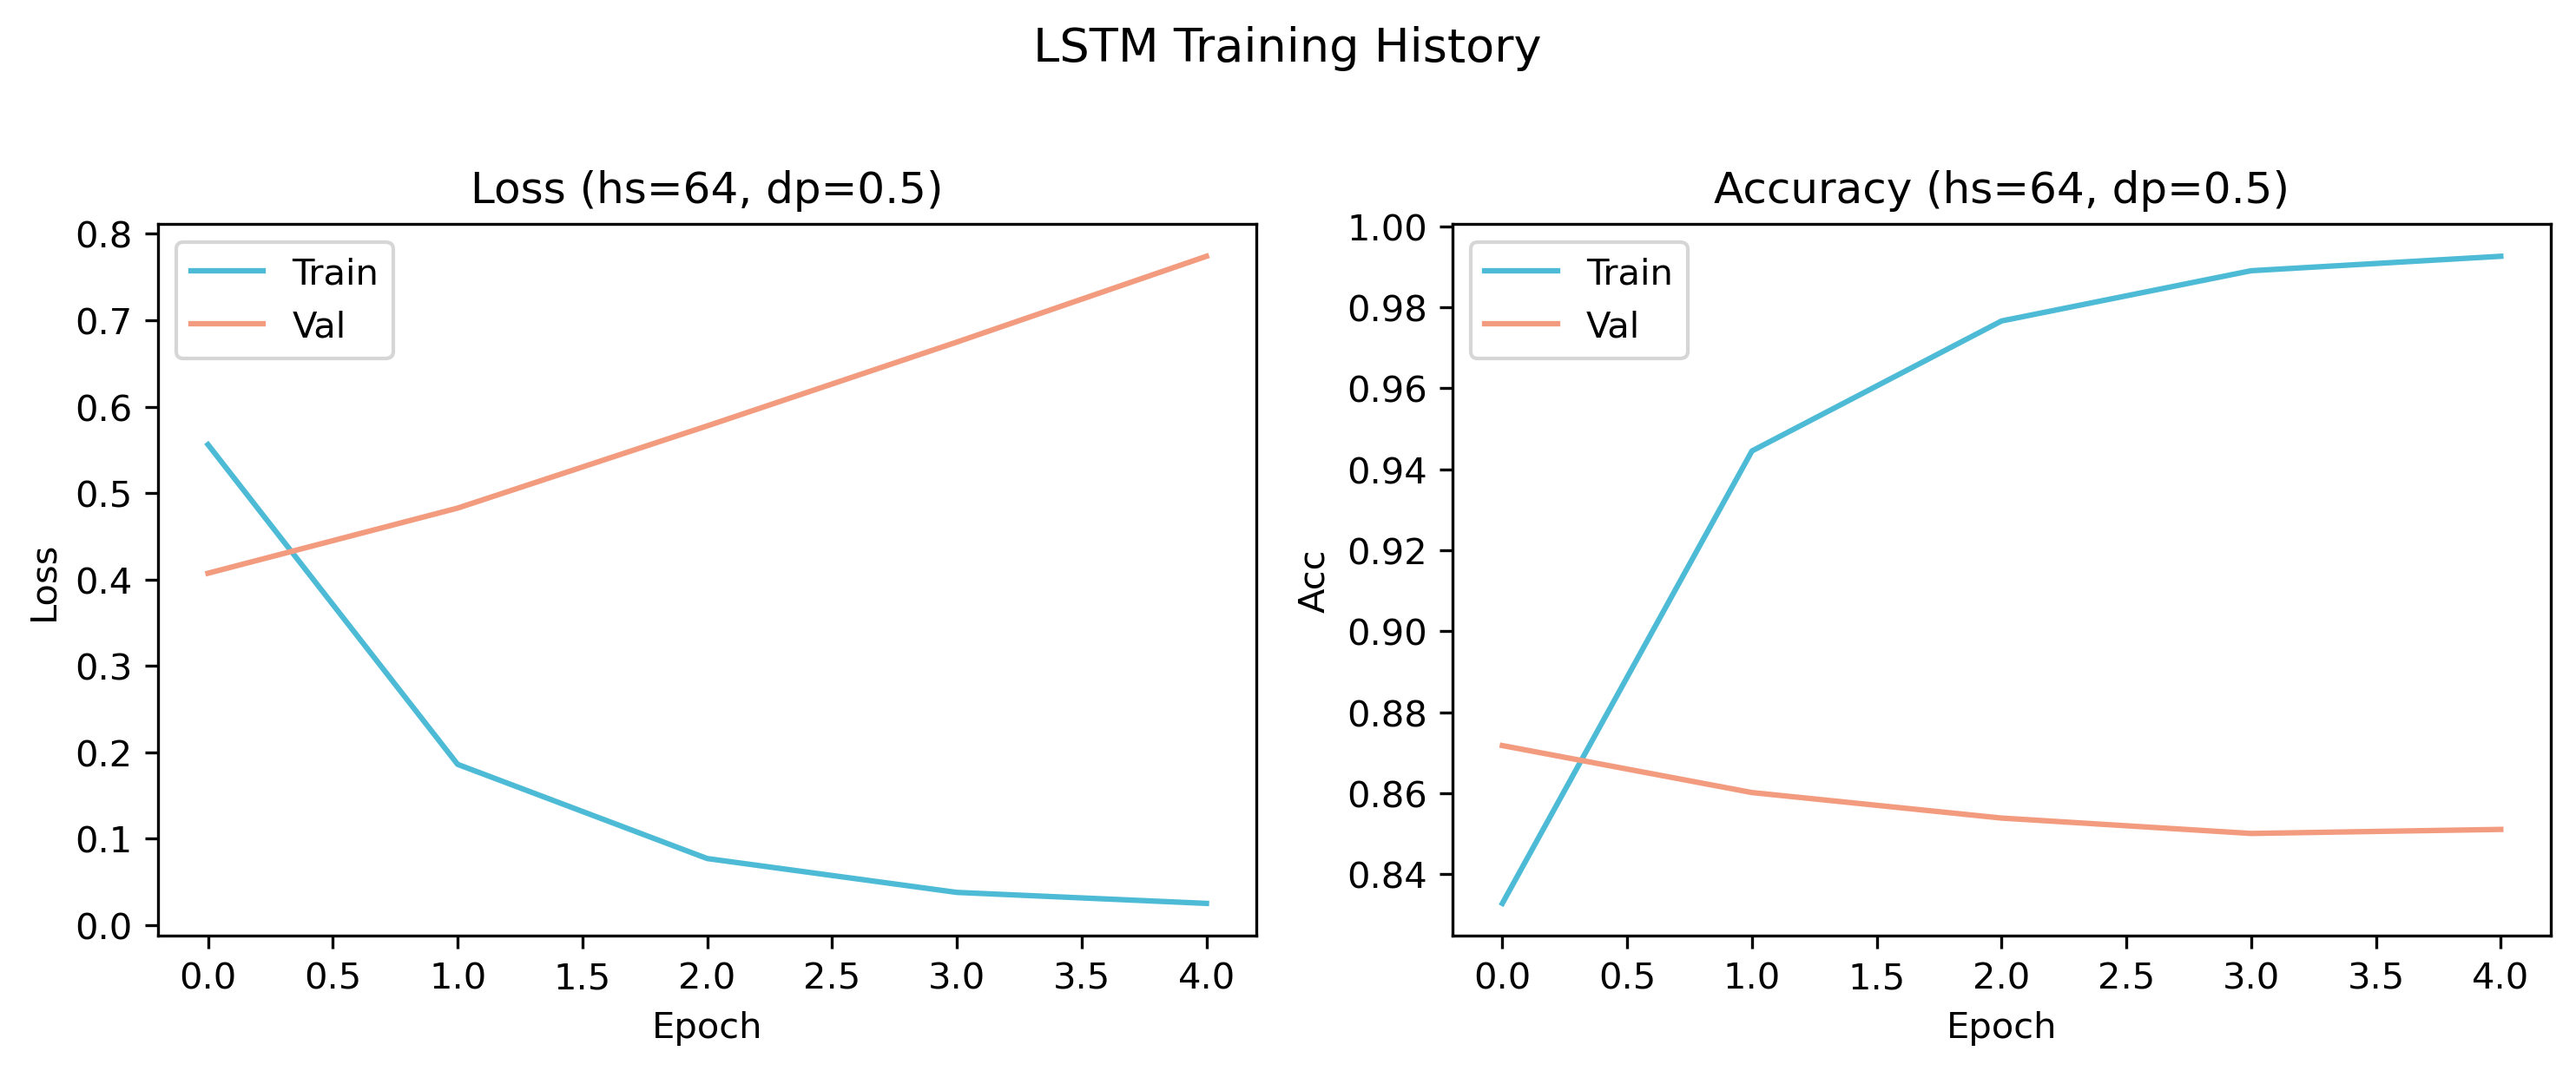
\includegraphics[width=\textwidth]{lstm_LSTM_h64_d0.5_curves.png}
\caption{LSTM 训练曲线}
\label{fig:curves}
\end{subfigure}
\begin{subfigure}[b]{0.46\textwidth}
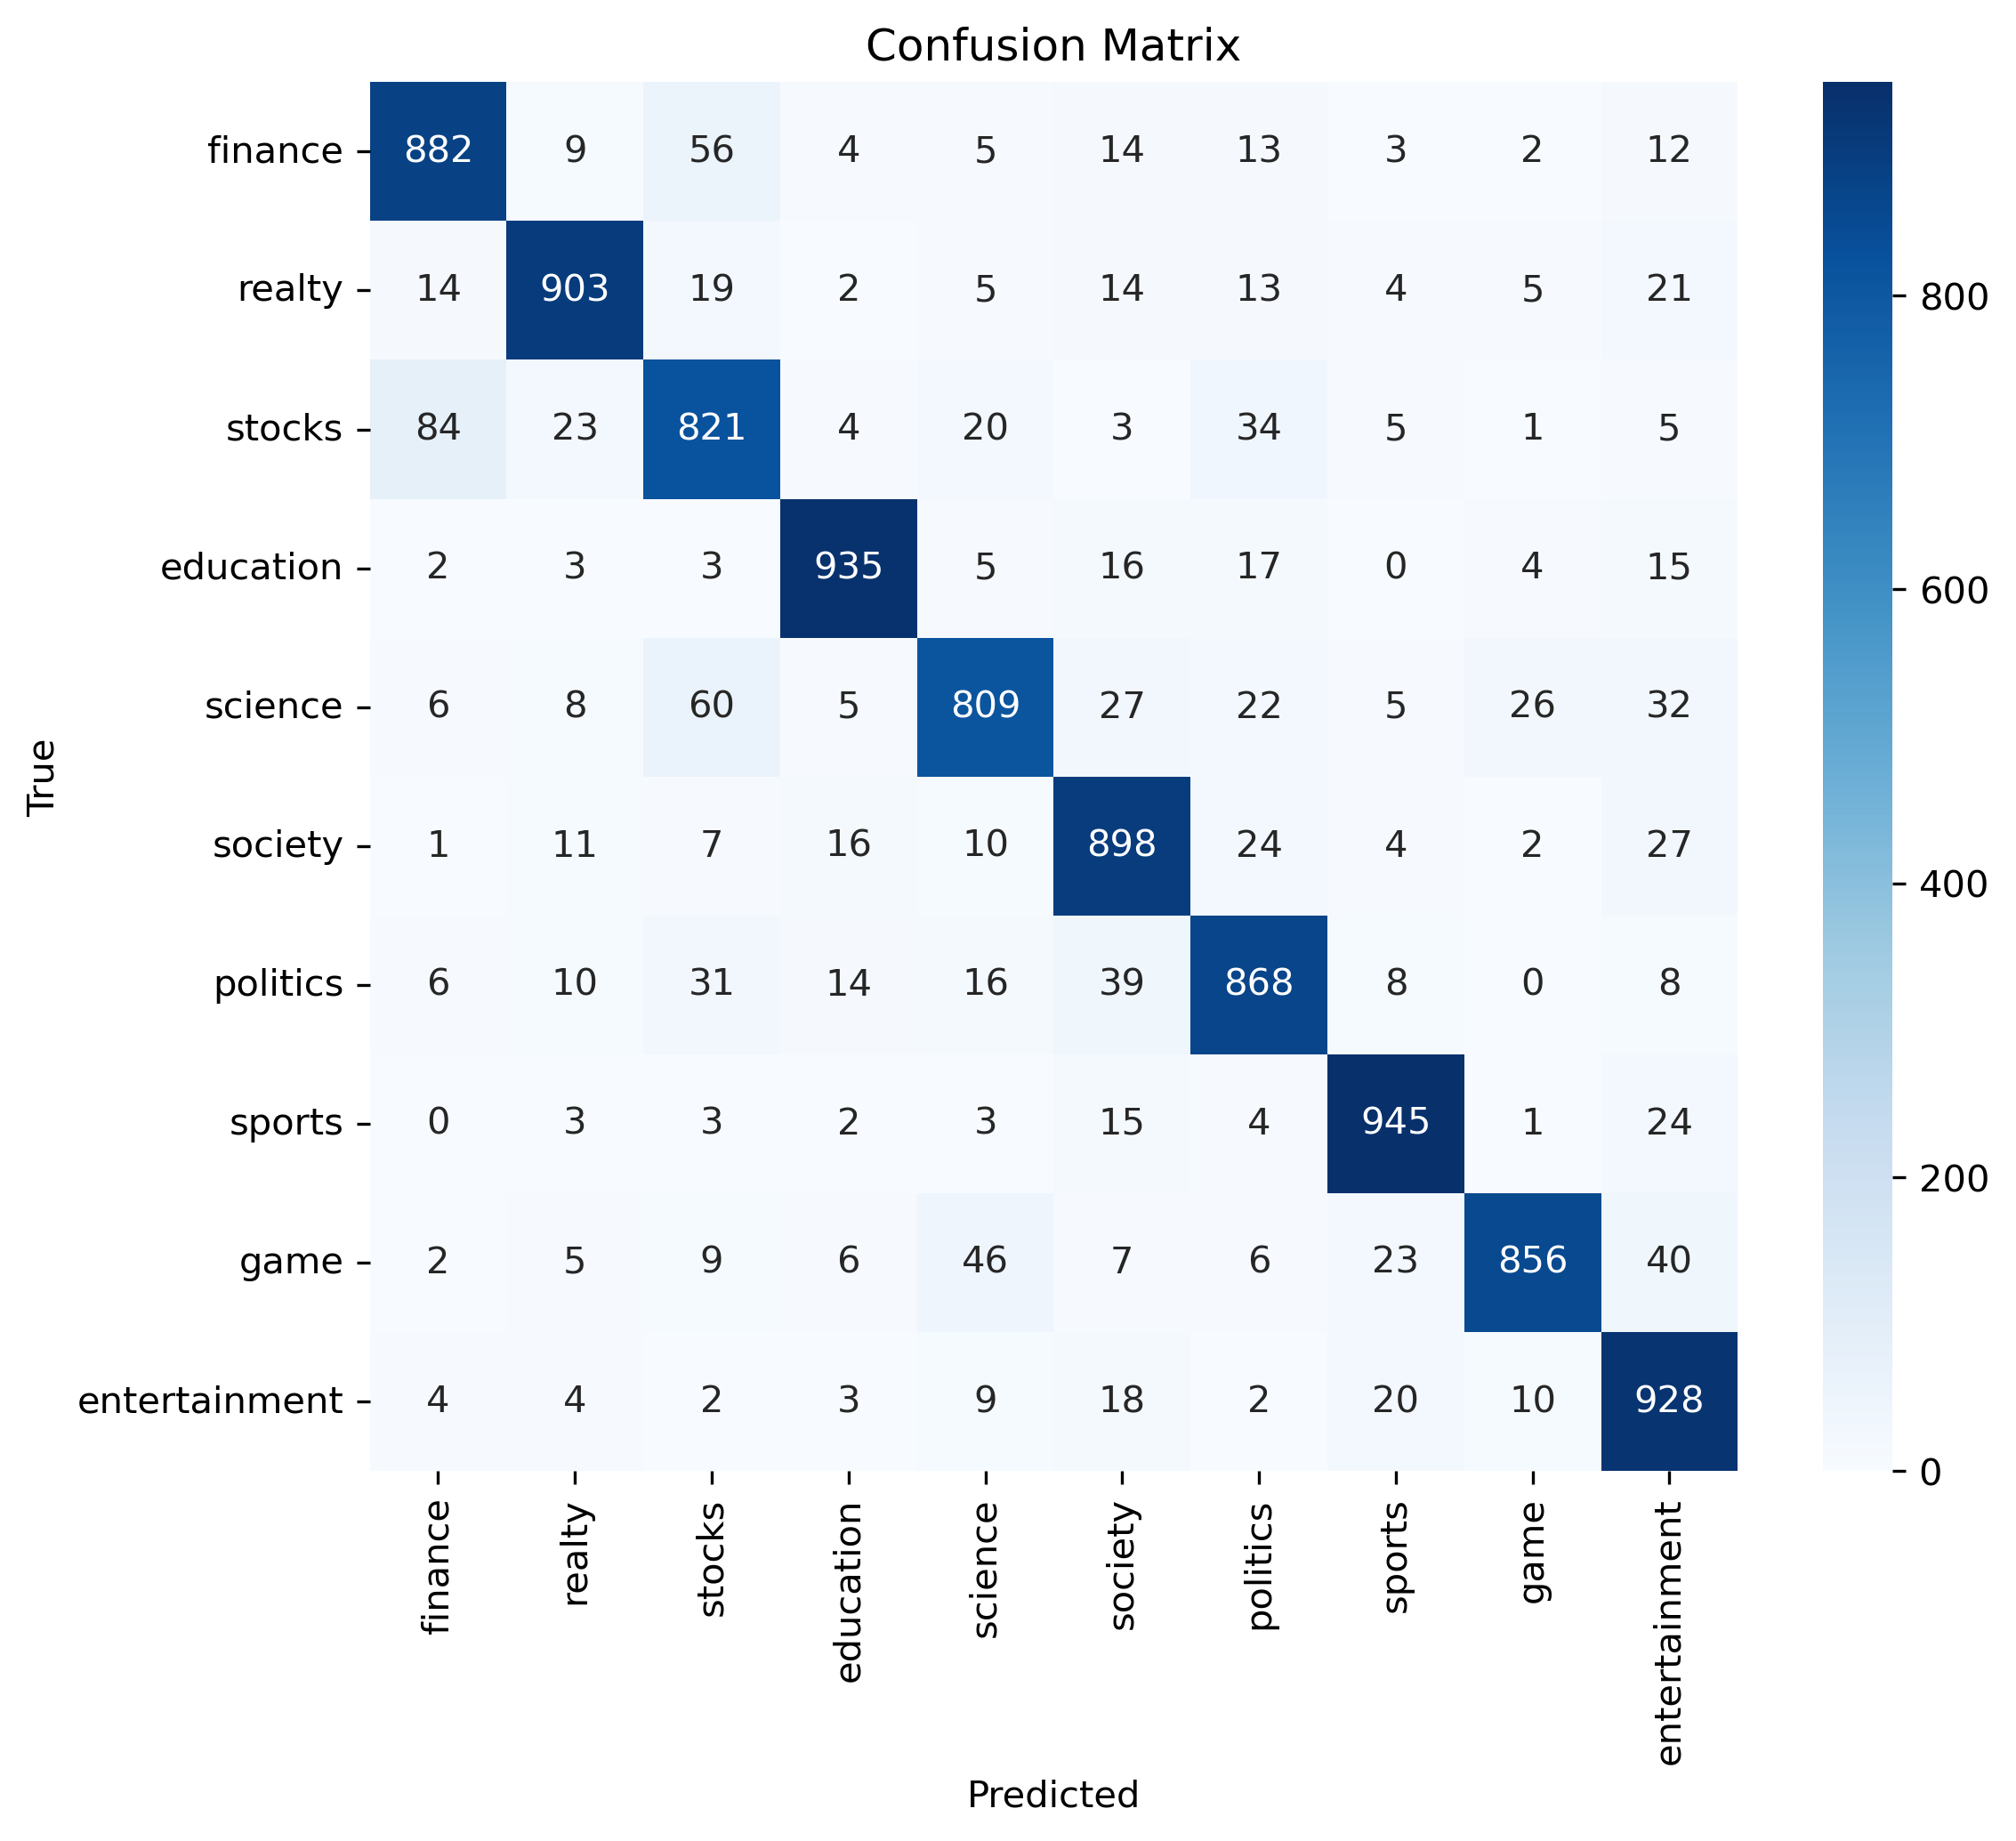
\includegraphics[width=\textwidth]{lstm_LSTM_h64_d0.5_confusion_matrix.png}
\caption{LSTM 混淆矩阵}
\label{fig:lstm_cm}
\end{subfigure}
\begin{subfigure}[b]{0.46\textwidth}
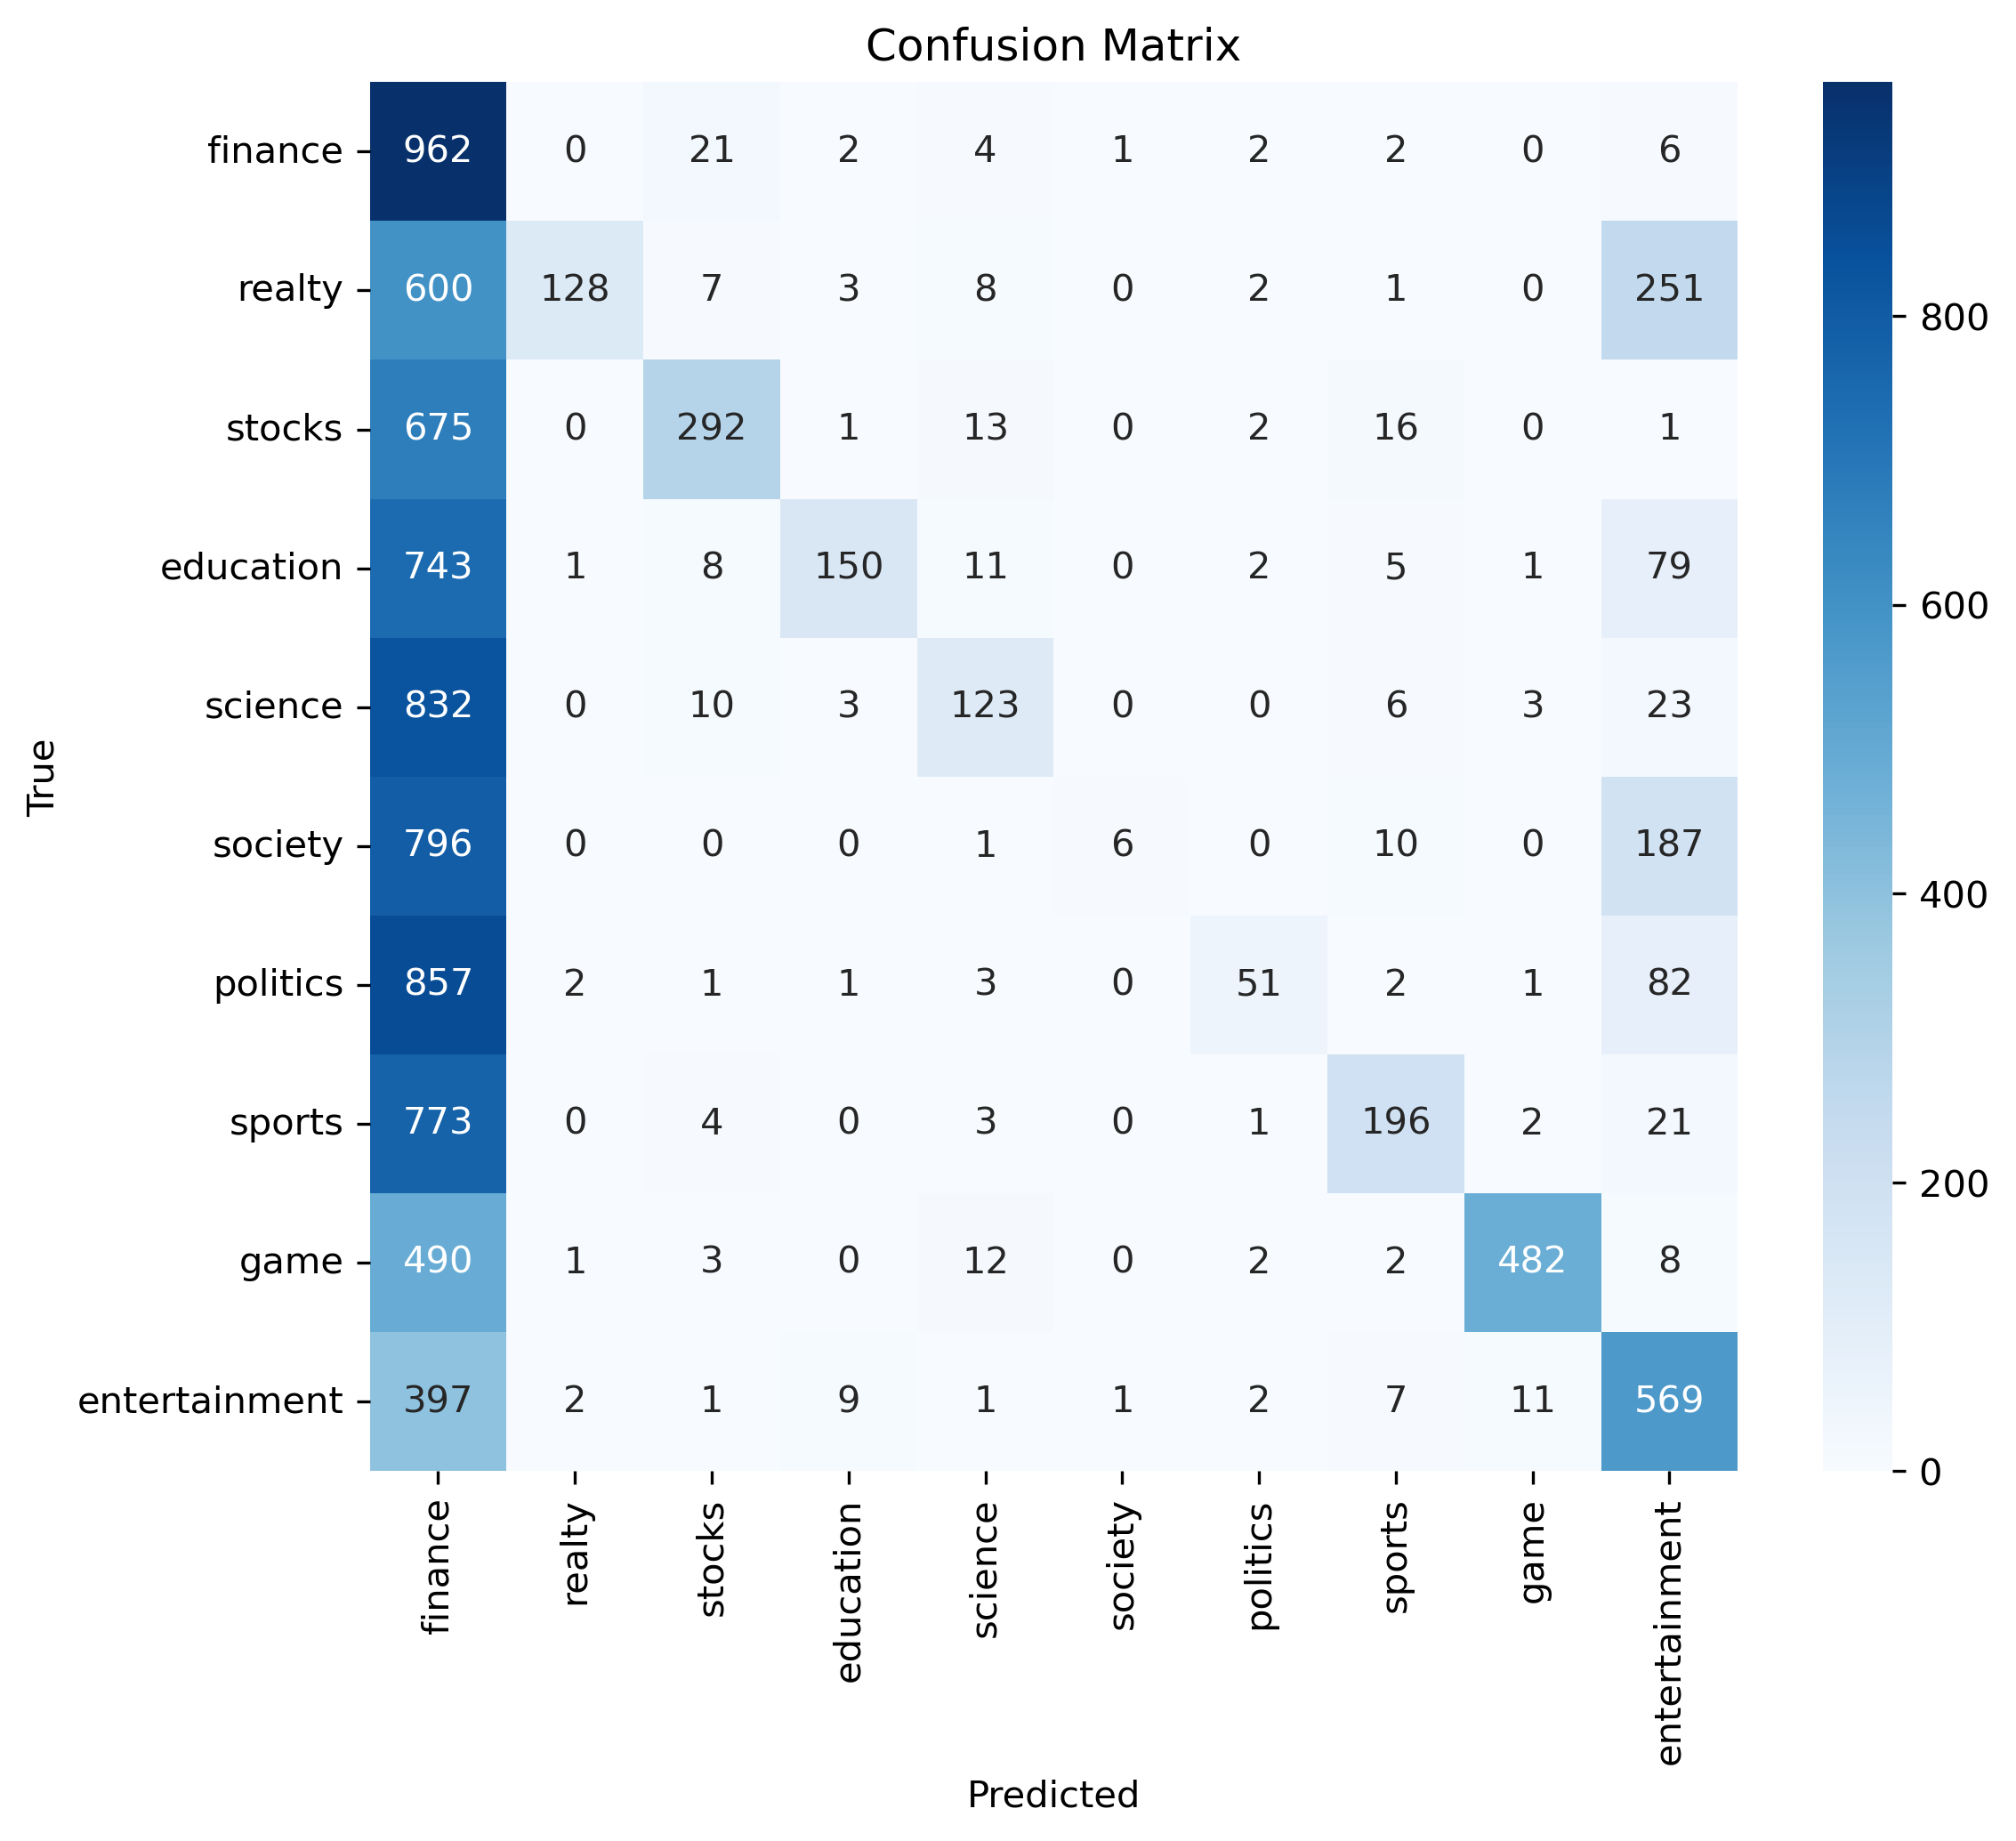
\includegraphics[width=\textwidth]{nb_confusion_matrix.png}
\caption{Naive Bayes 混淆矩阵}
\label{fig:nb_cm}
\end{subfigure}
\begin{subfigure}[b]{0.46\textwidth}
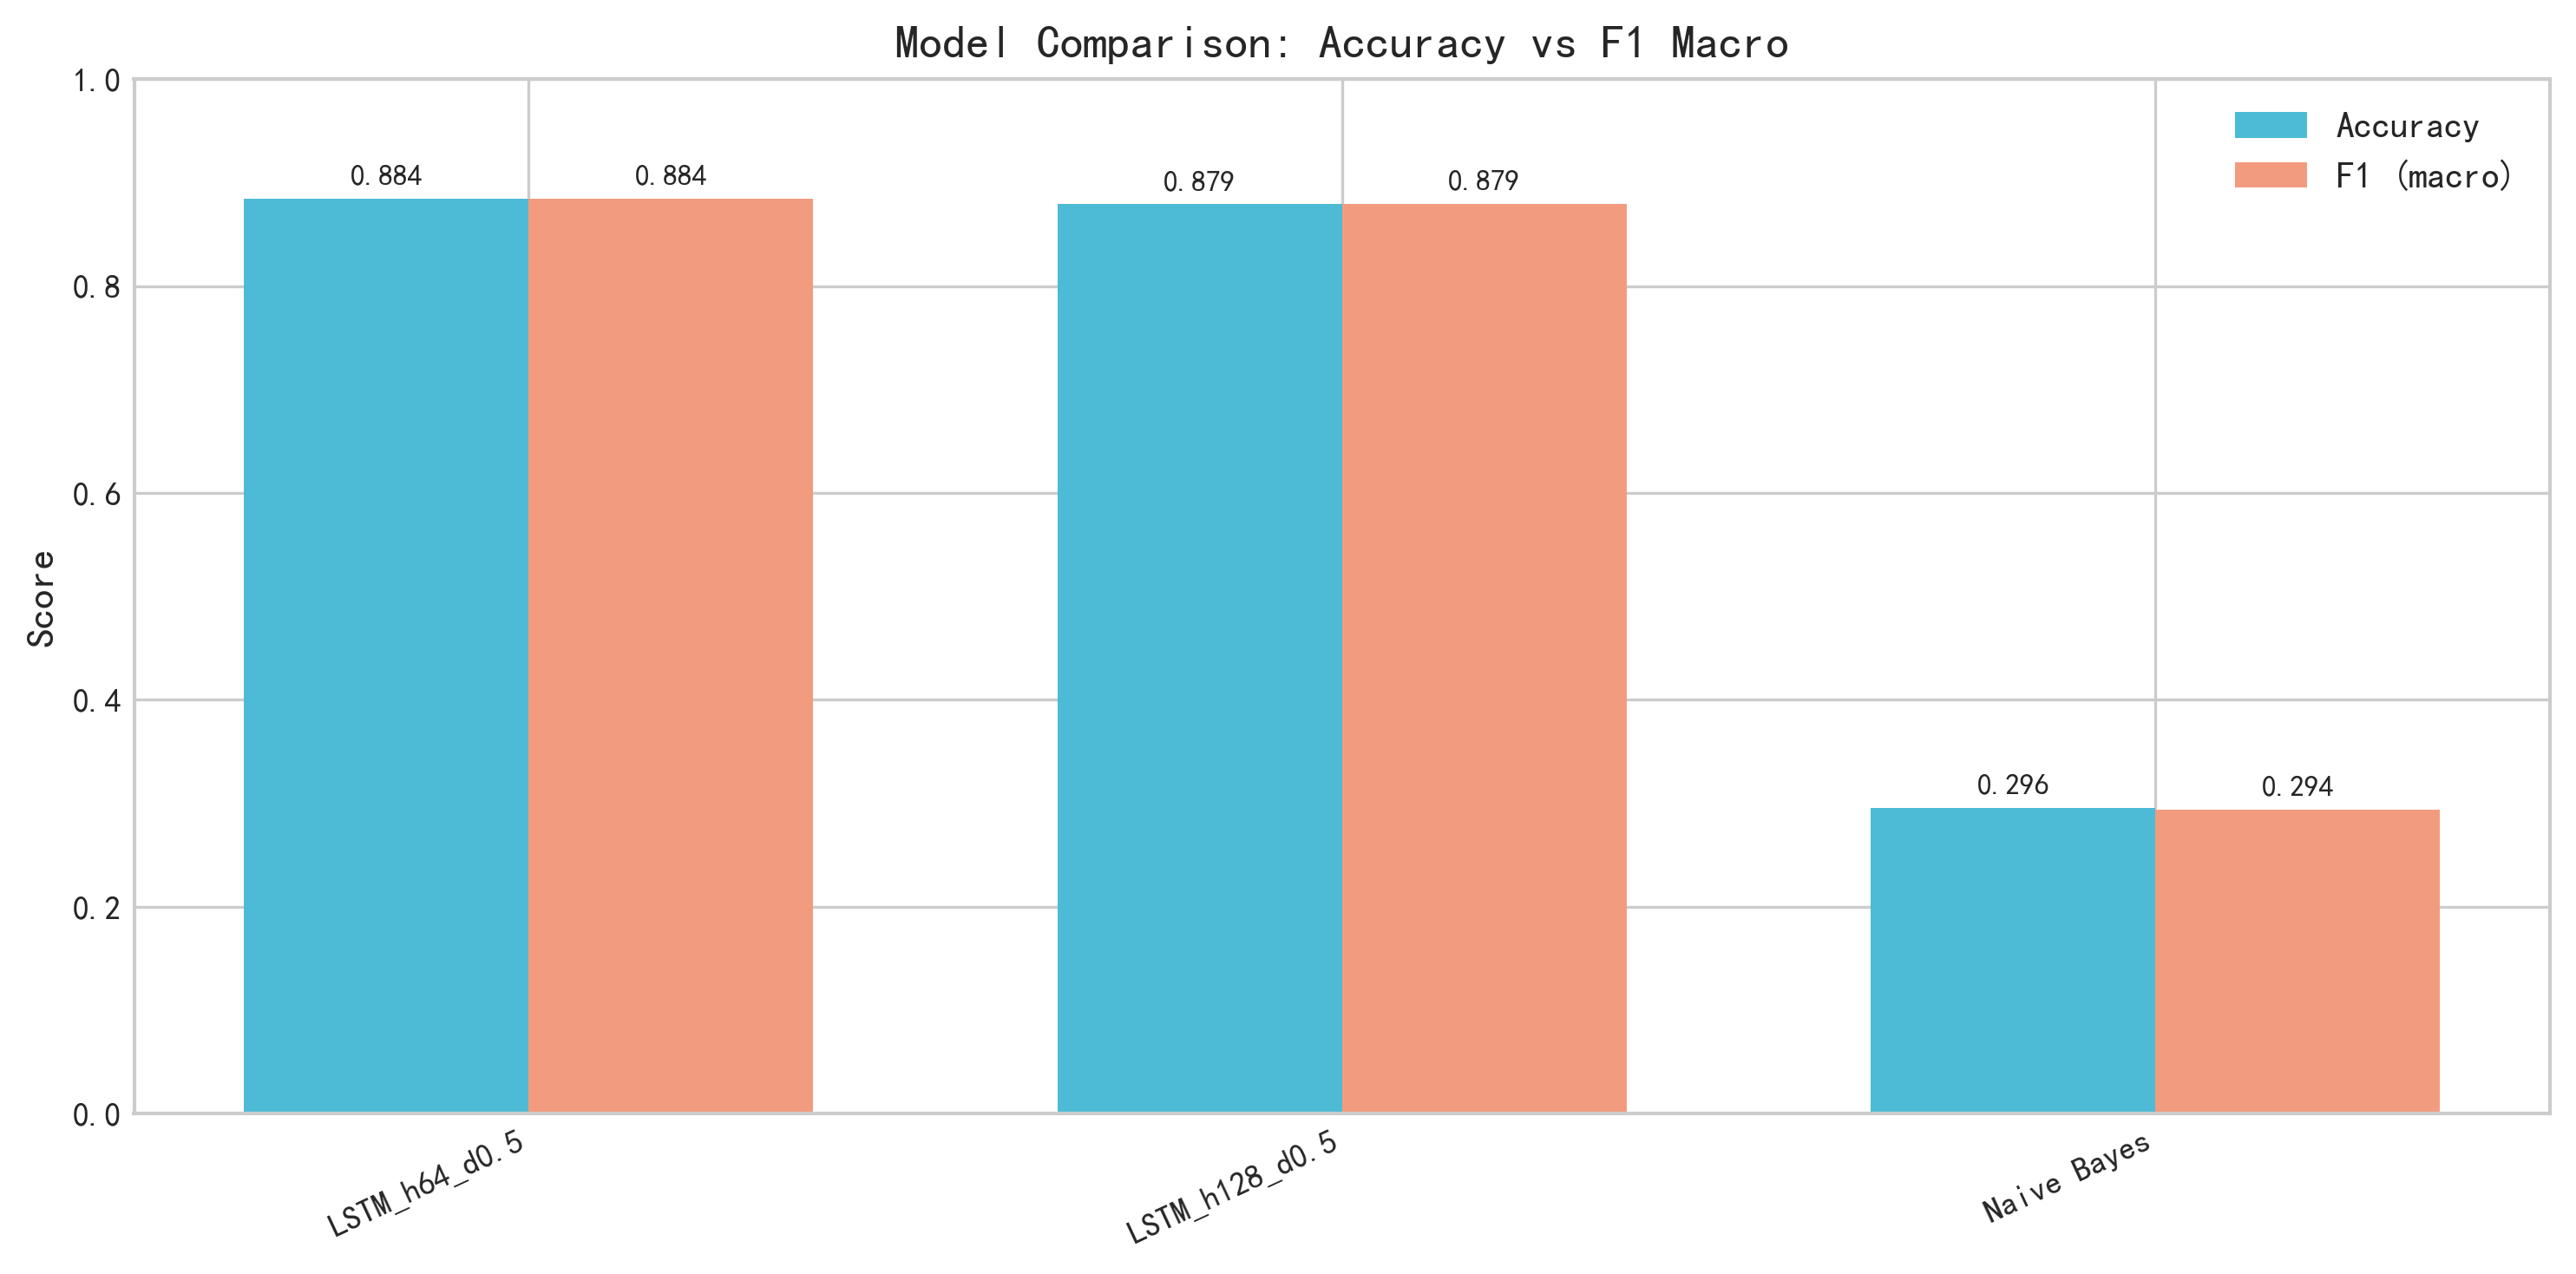
\includegraphics[width=\textwidth]{fig_model_comparison.png}
\caption{模型性能对比}
\label{fig:comparison}
\end{subfigure}
\caption{文本分类实验结果}
\label{fig:classification}
\end{figure}

图~\ref{fig:curves} 显示了 LSTM 最佳模型的训练曲线。模型在第一个 epoch 后训练准确率即达到 83.28\%，验证准确率达到 87.18\%，随后训练准确率持续上升至 99\% 以上，但验证准确率在第 1 轮后开始缓慢下降，出现了轻微的过拟合现象。早停机制在第 5 轮触发，保存了第 1 轮的模型作为最佳模型。这种快速收敛和较早的早停表明：(1) 预训练的 Word2Vec 词向量为模型提供了良好的初始特征表示；(2) 30{,}000 条训练子集足以使模型快速学习到类别间的判别特征。

图~\ref{fig:lstm_cm} 展示了 LSTM 最佳模型在测试集上的混淆矩阵。可以看出，模型在大部分类别上表现良好，对角线元素显著高于非对角线元素。分类错误主要集中在语义相近的类别之间，如 finance（财经）与 stocks（股票）的混淆（两者均涉及金融市场信息）、society（社会）与 politics（政治）的混淆（社会新闻与政治新闻在内容上常有重叠）。相比之下，Naive Bayes 的混淆矩阵（图~\ref{fig:nb_cm}）呈现出完全不同的模式：模型预测严重偏向于少数类别（如 science 和 society），大部分测试样本被归入这几类，导致其他类别的召回率极低。这种失衡源于朴素贝叶斯的特征独立性假设不适用于高维且词汇重叠严重的文本数据，使得模型难以准确区分各类别间的决策边界。图~\ref{fig:comparison} 则直观地对比了各模型的准确率和 F1 值，LSTM 显著优于 Naive Bayes 基线。

从模型复杂度来看，隐藏单元数从 64 增加到 128 并未带来性能提升（准确率从 88.45\% 下降至 87.90\%），反而增加了训练时间（从 87.6s 增至 143.0s）并加剧了过拟合。这表明对于 10 类短文本分类任务，64 维的隐藏状态已经足以捕捉有效的序列特征，更大的模型容量反而导致过拟合。进一步分析各类别的分类表现可以发现，sports（体育）和 science（科技）的 F1 值最高（均超过 0.92），而 realty（房产）和 stocks（股票）相对较低（约 0.85），这可能反映了前两类新闻具有更鲜明的领域关键词，而后两类与其他类别（finance、society）在词汇使用上存在较多重叠。

\subsection{情感分析结果}

对测试集 10{,}000 条样本进行情感分析的结果显示，正面情感样本占比 43.3\%，中性样本占 41.7\%，负面样本占 15.0\%。整体上以正面和中性新闻为主，负面新闻占比较低，这与中文新闻媒体的报道风格一致。

\begin{figure}[htbp]
\centering
\begin{subfigure}[b]{0.46\textwidth}
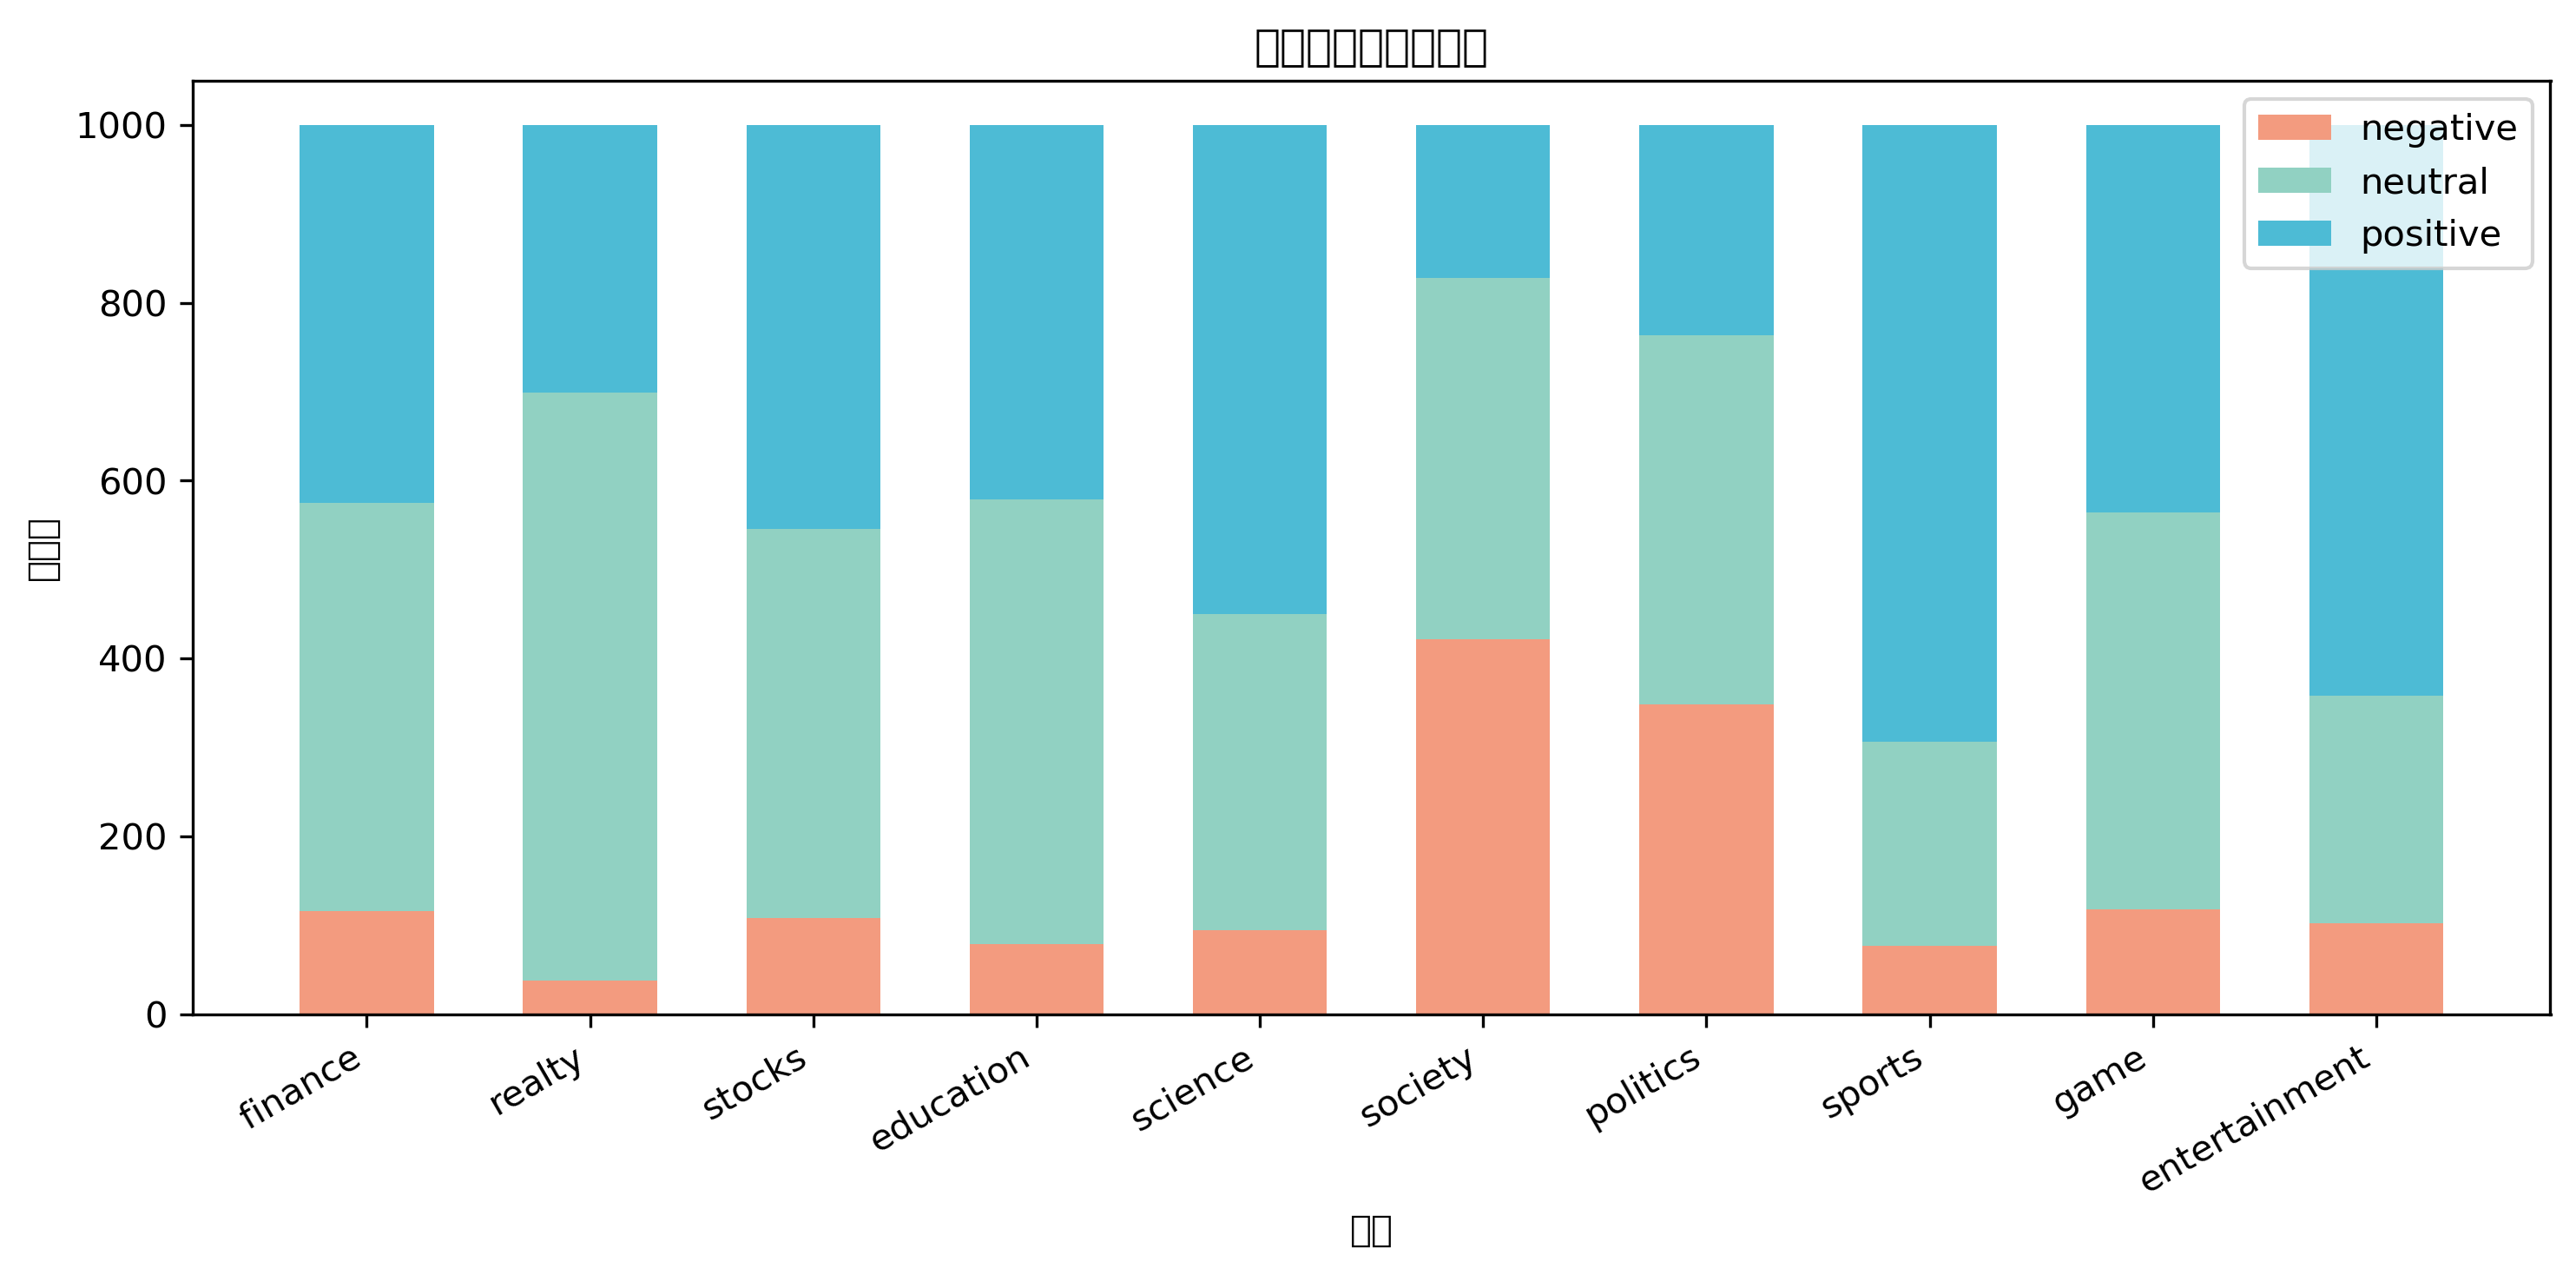
\includegraphics[width=\textwidth]{fig_sentiment_distribution.png}
\caption{情感极性分布（堆叠柱状图）}
\label{fig:senti_dist}
\end{subfigure}
\begin{subfigure}[b]{0.46\textwidth}
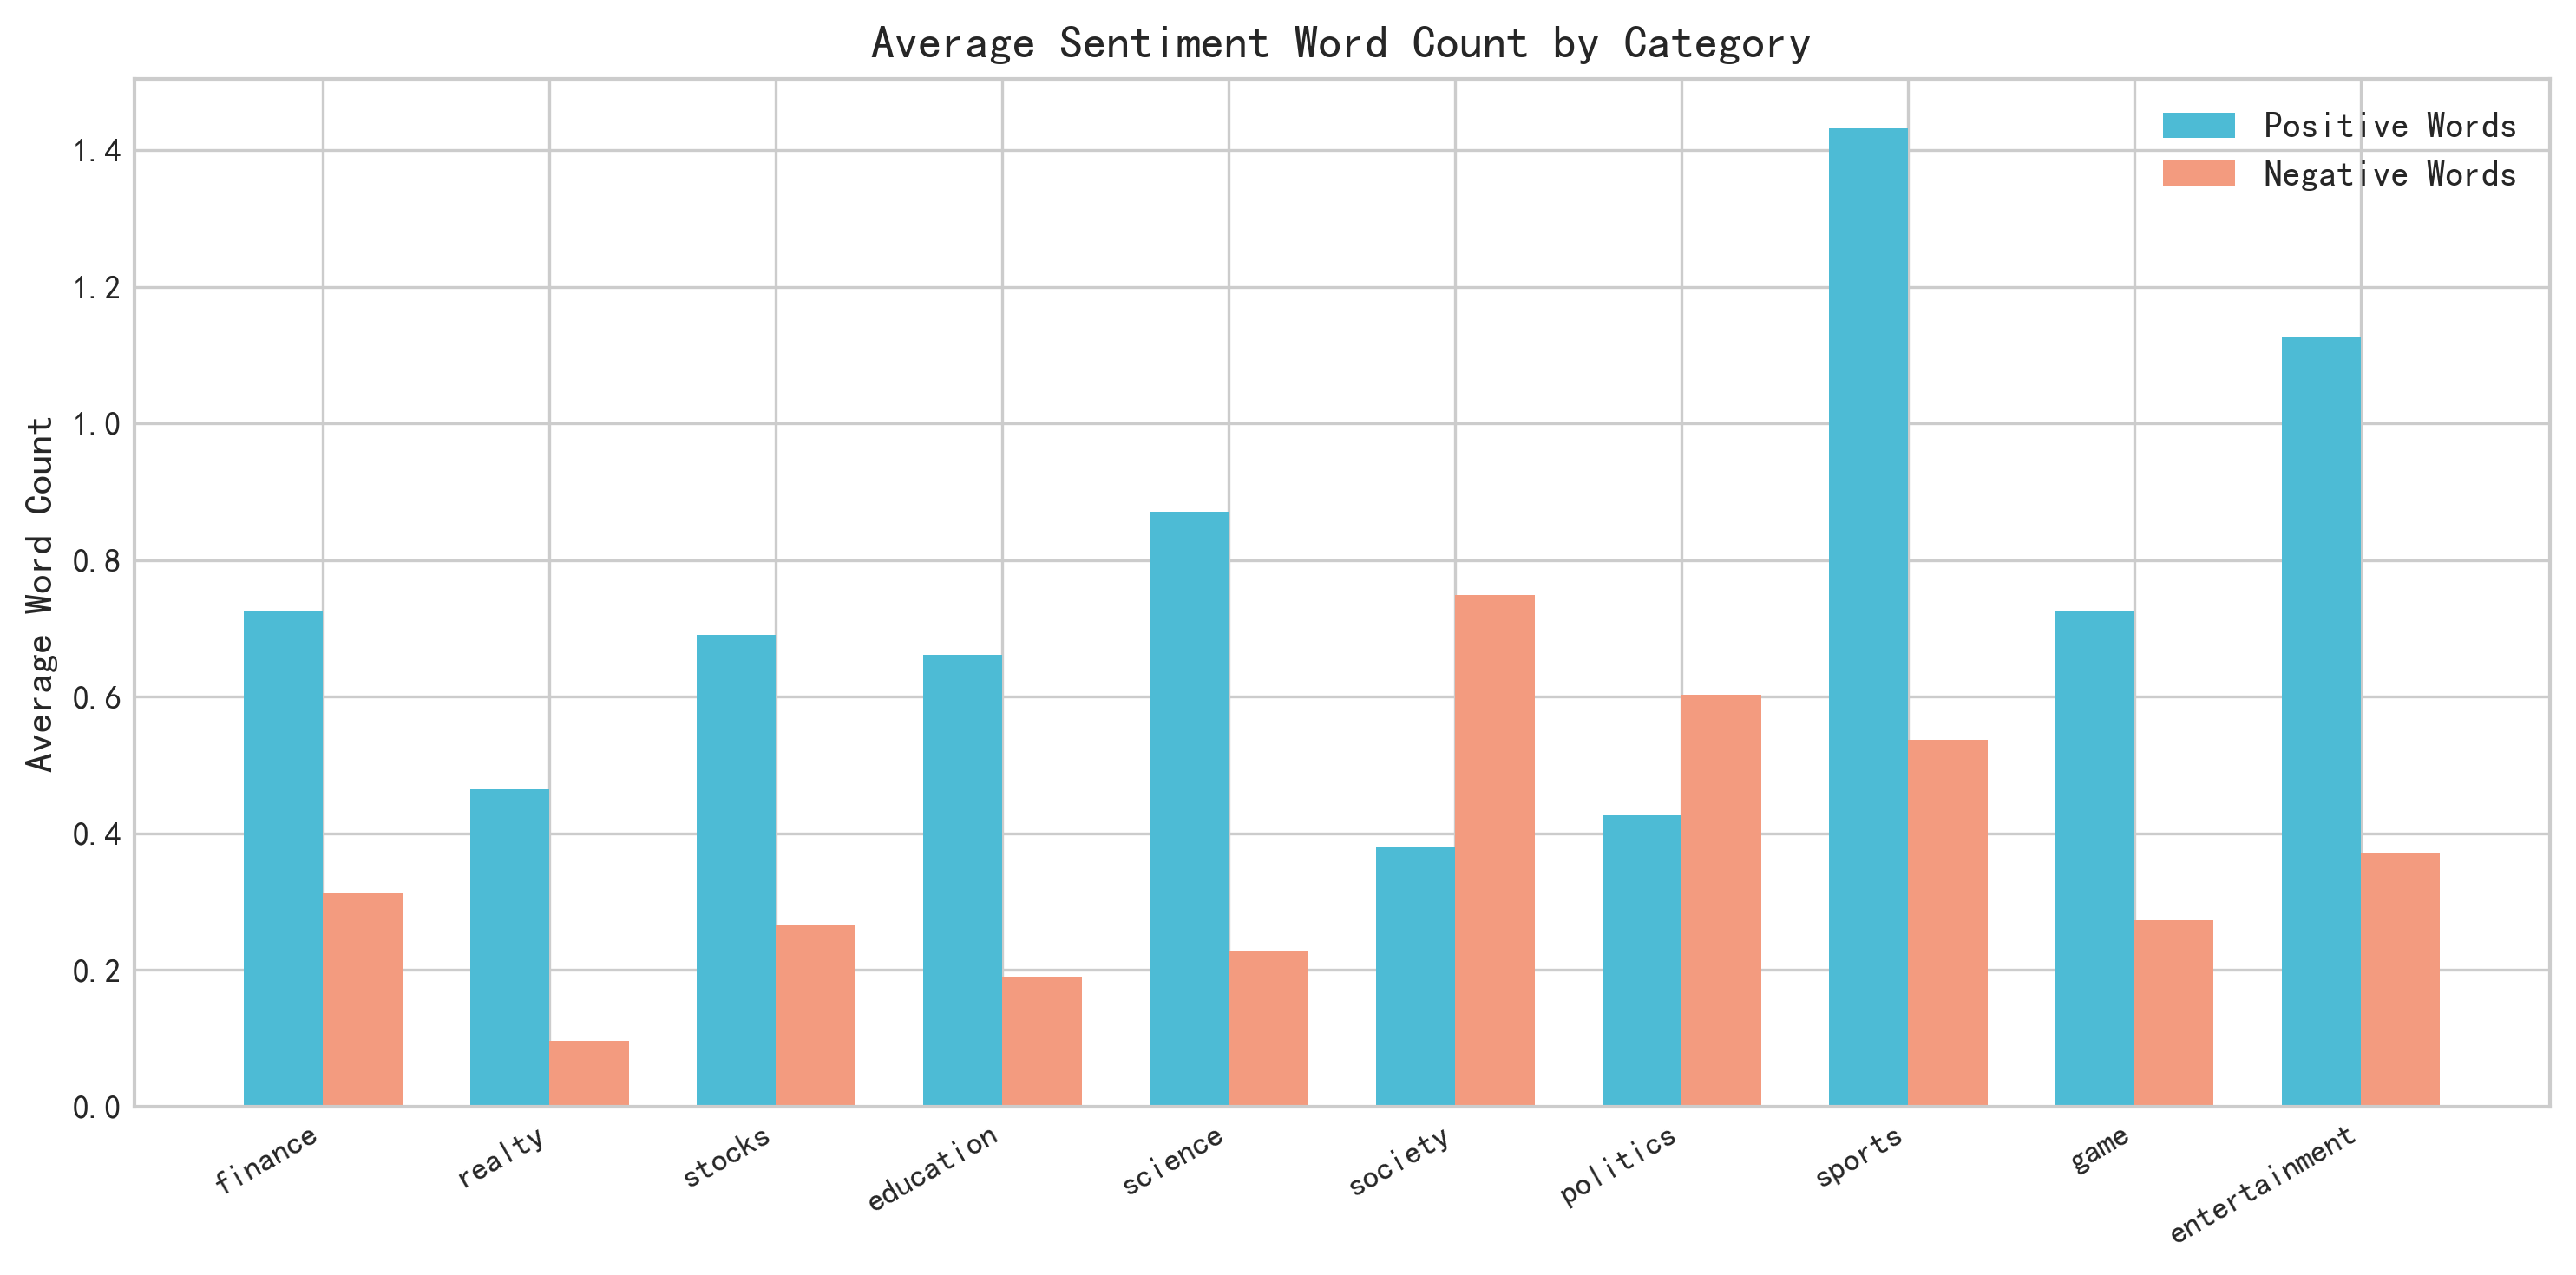
\includegraphics[width=0.78\textwidth]{fig_sentiment_by_category.png}
\caption{平均情感词数量}
\label{fig:senti_cat}
\end{subfigure}
\caption{情感分析结果}
\label{fig:sentiment}
\end{figure}

图~\ref{fig:senti_dist} 显示了各类别的情感极性分布。不同新闻类别的正面情感占比差异显著：sports（体育）的正面比例最高（69.4\%），这反映了体育报道多以取胜、突破等正面事件为主；entertainment（娱乐）次之（64.2\%），娱乐新闻以宣传和推广为主基调。而 society（社会）的正面比例最低（17.2\%），负面比例最高（42.2\%），因为社会新闻往往涉及灾难、犯罪等负面事件；politics（政治）亦负向偏高（34.8\%），这与政治新闻中包含较多争议性议题有关。值得注意的是，realty（房产）的中性比例高达 66.1\%，是最中性的类别，这可能与房产新闻多采用客观数据报道、较少使用情感词汇的风格有关。

图~\ref{fig:senti_cat} 从情感词数量的角度呈现了相同的趋势：sports 和 entertainment 的平均正面情感词数量显著高于其他类别，而 society 和 politics 的平均负面情感词数量最高。

\subsection{分类与情感分析综合对比}

将文本分类结果与情感分析结果综合来看，可以发现一个有趣的模式：分类准确率较高的类别（如 sports 的 88.45\% 正面对应 69.4\% 正面情感、entertainment 的 87.90\% 正面对应 64.2\% 正面情感）同时也是正面情感占比最高的类别。相反，负面情感占比最高的 society（42.2\% 负面）虽然分类准确率仍有 87\% 左右，但略低于最佳类别。这种关联性表明，正面报道较多的领域可能具有更加鲜明和一致的语言特征，有利于分类器进行识别；而负面报道集中的领域可能由于情感词汇带来的语义干扰，对分类性能产生轻微影响。

从方法层面来看，LSTM 的高分类准确率（88.45\%）与基于词典的情感分析之间形成了有趣的对比。LSTM 通过有监督学习从标注数据中自动提取特征，能够学习到类别间的细微语义差异，因此分类性能较高。而基于情感词典的方法无需训练数据，完全依赖人工构建的词典进行词级匹配，虽然无法达到深度学习的分类精度，但其优势在于可解释性强——每一条文本的情感判定都可以追溯到具体的情感词汇，情感分析的结论易于理解和验证。

此外，情感分析的结果还揭示了一个值得关注的发现：不同新闻类别在情感分布上的差异远比分类任务所反映的更为丰富。例如，finance 和 stocks 在分类任务中容易相互混淆（语义相近），但在情感分析中却呈现出不同的情感特征——stocks 的正面占比（45.4\%）高于 finance（42.5\%），这可能反映了股市报道中"上涨"、"盈利"等正面词汇的使用频率高于综合财经报道。

% ============================================================
\section{结论}
% ============================================================

本文以 THUCNews 中文新闻数据集为对象，开展了一项结合文本分类与情感分析的对比研究。在文本分类方面，LSTM 模型取得了 88.45\% 的测试准确率，显著优于 Naive Bayes + TF-IDF 基线（29.59\%），验证了深度学习模型在中文短文本分类任务中的有效性。实验还表明，64 维的 LSTM 隐藏状态对于 10 类分类任务已足够，更大的模型容量并不能带来性能提升。在情感分析方面，基于 DUTIR 情感词典的分析揭示了不同新闻类别的情感分布差异：体育和娱乐类正面情感突出（69.4\% 和 64.2\%），社会和政治类负面情感较多（42.2\% 和 34.8\%）。综合对比发现，正面情感占比较高的类别往往也取得更好的分类性能，提示类别的情感特征与可分类性之间存在一定关联。具体而言，sports 和 entertainment 等正面报道为主的类别在分类准确率和情感正面率上均领先，而 society 等负面事件集中的类别虽然分类性能仍可接受，但情感分析的负面占比明显偏高，说明情感信息可以作为分类任务之外的补充维度。此外，在区分语义相近的类别（如 finance 和 stocks）时，情感分析的差异化结果（stocks 正面率 45.4\%，finance 正面率 42.5\%）为细粒度类别分析提供了新的视角。

本研究的不足在于：(1) LSTM 模型仅在 30{,}000 条采样数据上训练，若能使用全量数据并结合 GPU 加速，预期可进一步提升性能；(2) 情感分析仅采用了词典方法，未与基于模型的情感分析方法进行对比。后续工作可考虑使用预训练语言模型（如 BERT）进行文本分类，并探索基于深度学习的情感分析模型以获得更丰富的情感分析结果。

\end{document}
